\chapter{Implementation}
\renewcommand{\baselinestretch}{\mystretch}
\label{chap:Fuzzer}
\PARstart{T}{ool} flow framework and grey-box fuzzing algorithm are two implementations of this project. This chapter will illustrate the detailed Linux Shell and C++ code programming with a flowchart of each block (embedded, general, FSM et al.). The code implementation of this project inspired by Jeffrey designed security architecture \cite{dwoskin2010framework} and Clifford designed VlogHammer \cite{clifford}. 
\section{Toolflow}
Linux shell script is an effective way to control tool-flow. Two scripts with embedded architecture are used in the project. The top-level script is \texttt{time.sh}. The embedded sub-script is \texttt{check\_ABC.sh} which is used to perform ABC checking process. Following sections will illustrate them separately. 
\subsection{\texttt{time.sh}}
\begin{figure}[htb]
    \centering
    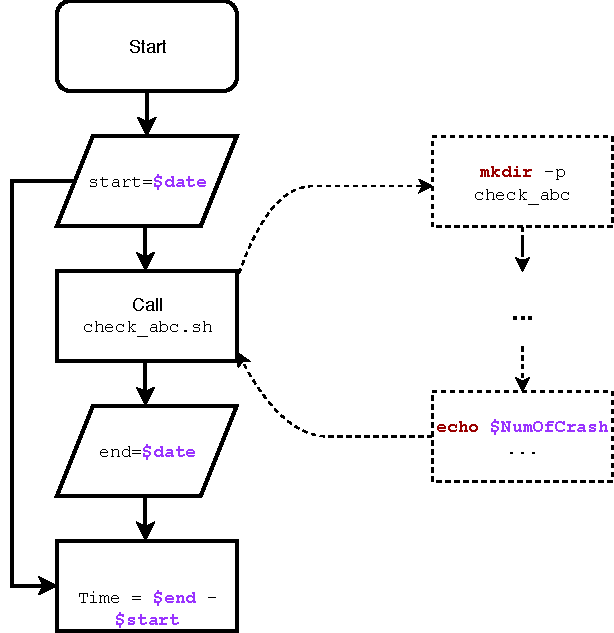
\includegraphics[scale=0.8]{MScThesisTemplate/Figs/time_sh.pdf}
    \caption{\footnotesize Flow chart of \texttt{time.sh}}
    \label{fig:time.sh}
\end{figure}
As shown in above flow chart, the solid line represents states of \texttt{time.sh} script and the dashed line represents states of sub-script \texttt{check\_abc.sh}.  Two variables were defined to record real system time in the beginning and the end of sub-script running to obtain the runtime of checking  ABC. $\%N$ is utilised to produce a result in nanosecond level precision. However, the calculated result sometimes may exceed the maximum digit limitation. 
\subsection{\texttt{check\_abc.sh}}
Flowing the designed basic framework \ref{fig:arch}, there is only one DUT: ABC. First step is to use Linux \texttt{mkdir} command in creating a empty file to store EC result \texttt{.txt} files. The following step is to initialise three counting variables those used to record the number of crashes, the number of equivalence check (EC) passed, and the number of EC failed. A\texttt{for} loop would be applied to perform iteration in injecting Verilog files to ABC and obtaining feedback information. 

In each iteration, ABC executes in its batch mode with pre-assigned commands. ''\texttt{rv}'' is an abbreviate alias of ''\texttt{read\_verilog}''. After reading the Verilog file, ABC would perform circuit optimisation. Table \ref{tab:abc commands} shows ABC's circuit optimisation commands. Next, the equivalence of original input Verilog file and optimised netlist would be checked by an equivalence checker. The checking report would be writtten to pre-allocated \texttt{.txt} file. Then, the information of \texttt{.txt} file would be extract to terminal by Linux \texttt{grep} command. It will be used in case judgement to increase the corresponding counting variable. When achieves the user-defined iteration number, \texttt{for} loop will be terminated and print the testing result on-screen using \texttt{echo} commands.
\begin{table}[htb]
    \centering
    \begin{tabular}{c|c}
    \hline
         Combinational optimisation&Sequential optimisation  \\
         \hline
         balance & (strash) cycle\\
         (strash)renode&(strash) retime\\
         cleanup&(strash) scleanup\\
         sweep&(strash)xsim\\
    \end{tabular}
    \caption{\footnotesize ABC's circuit optimisation commands}
    \label{tab:abc commands}
\end{table}

\begin{figure}[htb]
    \centering
    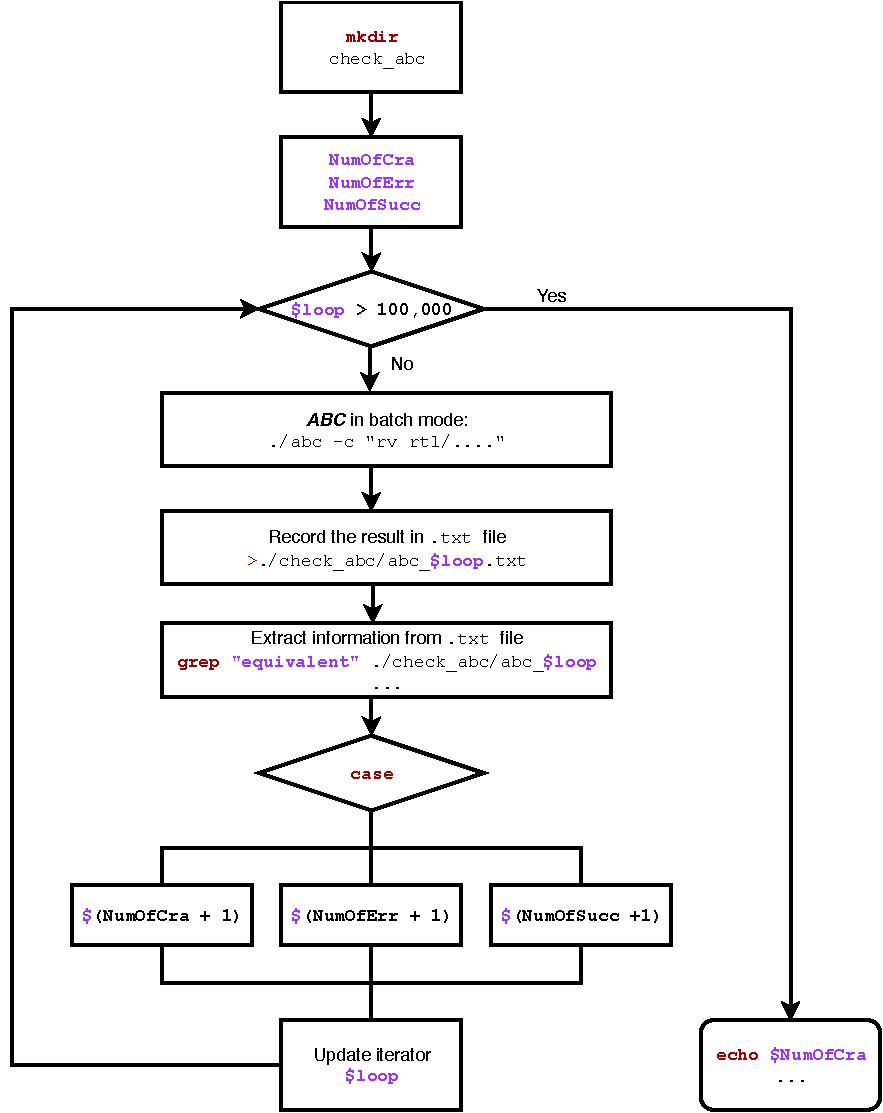
\includegraphics[width=10cm]{MScThesisTemplate/Figs/check_abc.pdf}
    \caption{\footnotesize\texttt{check\_abc.sh}}
    \label{fig:check_abc}
\end{figure}


\subsection{\texttt{check\_abc\_sis.sh}}
\texttt{check\_abc\_sis.sh} script is an implementation of architecture \ref{fig:arch_sis}. Compared to above framework, the number of DUT is increased. The initialisation and loop structure is the same as the previous \texttt{check\_abc.sh}. Different from the previous design, a format converter is placed before the parallel file injection to two DUTs: ABC and SIS. ABC's structure hashing function (\texttt{read\_verilog},\texttt{write\_blif})was called to convert the format without any circuit optimisation. Then, the converted BLIF file would be passed to ABC and SIS in parallel. The circuit optimisation commands of SIS are shown in following Table \ref{tab:sis commands}. Rest parts of this checking framework are similar to the previous DUT framework. In the final EC, these three files (original input Verilog, netlist from ABC and netlist from SIS) are compared in pairs to include following case judgement. The \texttt{NumOfSucc} would be increased only when detected ''equivalence'' from the reports of all three EC. If an error or crash was recorded, it might need manual analysis of its inducement.  
\begin{figure}[htb]
    \centering
    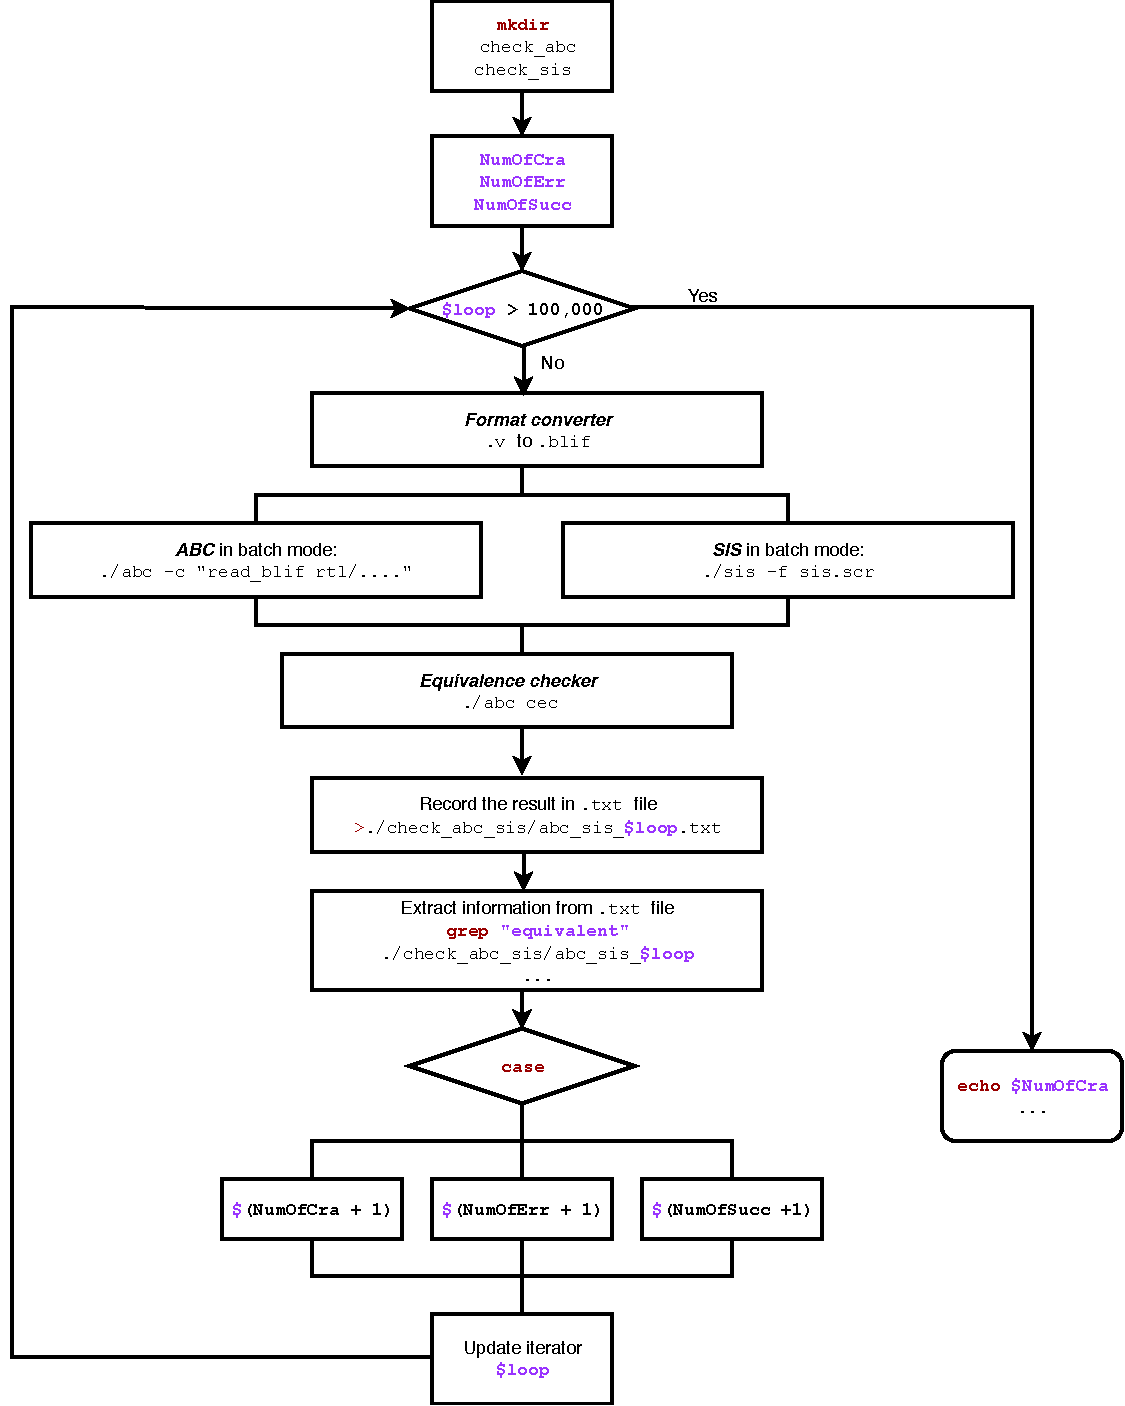
\includegraphics[width=10cm]{MScThesisTemplate/Figs/check_abc_sis.pdf}
    \caption{\footnotesize\texttt{check\_abc\_sis.sh}}
    \label{fig:check_sis}
\end{figure}

\begin{table}[htb]
    \centering
    \begin{tabular}{c|c}
    \hline
         Combinational optimisation&Sequential optimisation  \\
         \hline
         simplify & \multirow{2}{*}{retime}\\
         resub&\\
         speed\_up& \multirow{2}{*}{remove\_latch}\\
         reduce\_depth&\\
    \end{tabular}
    \caption{\footnotesize SIS's circuit optimisation commands}
    \label{tab:sis commands}
\end{table}
\section{Grey-box fuzzer}
In order to illustrate detail implementation processes of grey-box fuzzer, this section is divided into three subs: Global environment with main function, combinational and sequential implementation.
\subsection{Global environment with main function}
For maximum variety and efficiency of generation, grey-box fuzzer offers options to the user. The user could define the desired amount of Verilog and its type. This is implemented by C++ \texttt{\#define} and \texttt{\#undef} syntax in main function of this fuzzer. The functions and constant arrays contained in global environment shows in Fig. \ref{fig:global}. RNG produces a 32-bit random number by shifting and \textit{XOR}ing the seed. The statement in C++ is: ''\texttt{x \^{}  = x << 11;}''. As described in design chapter\ref{Global design}, the randomly generated number would be used to guide the printing functions. Defined print function would randomly print different Verilog statements those fetched from constant arrays by using C++ ''\texttt{fprint()}''.
\begin{figure}[htb]
    \centering
    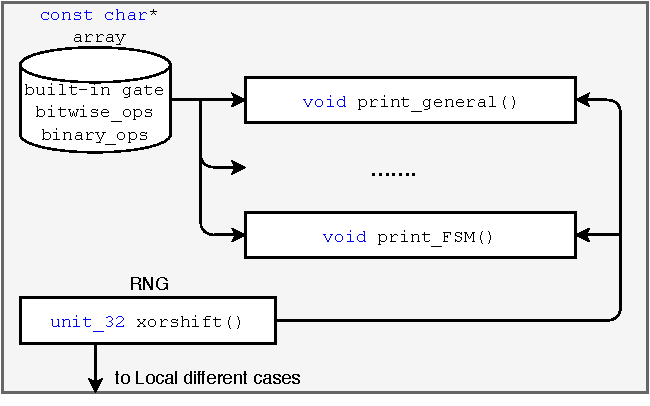
\includegraphics{MScThesisTemplate/Figs/Global.pdf}
    \caption{\footnotesize Global environment}
    \label{fig:global}
\end{figure}

\subsection{Combinational}
Three types of combinatial circuit were implemented in this project, \texttt{general.v}, \texttt{embedded.v} and \texttt{longer.v}. Basic implementation approach follows the local environment design flow chart \ref{fig:local}. 
\begin{figure}[htb]
    \centering
    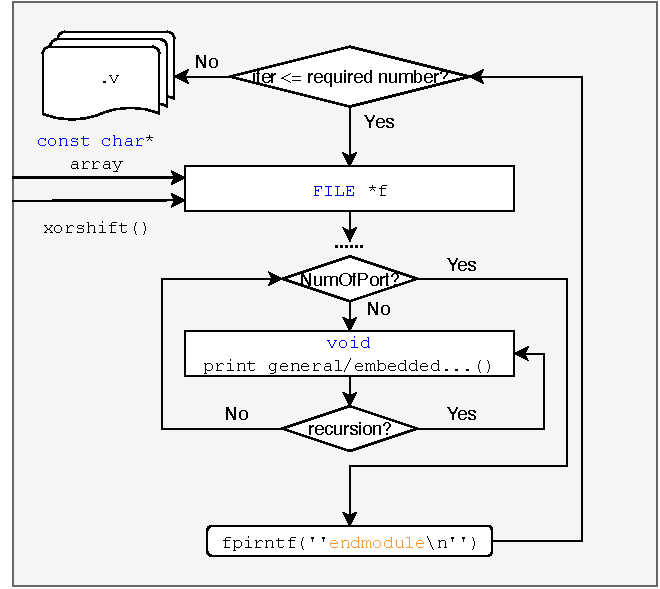
\includegraphics{MScThesisTemplate/Figs/local.pdf}
    \caption{\footnotesize Local environment}
    \label{fig:local}
\end{figure}
\subsubsection{\texttt{general.v}}
New Verilog file keeps being created until the number reaches the user's requirement. C++ file pointer ''\texttt{FILE *f}'' would allocate space from OS. All of the generated Verilog files will be gathered under a file called ''rtl''. In each file creation, RNG is called to produce a large random number. Using the modulus operator ''\%' to obtain a random number of input ports within 10. C++ statements is: ''\texttt{xorshift()\%10}''. The following step is execute module name, port declaration etc. unconditional printing. The output logical is a random combination of input ports and Verilog operators. The number of output ports is assigned three times of the number of input ports. For example, '\texttt{assign y = a1 || b2}''. The Verilog conditional statement ''\texttt{? : }'' and  cascade operator satisfies requirements of recursive call. If the recursion case is entered, printing function will call itself until dumping variable reaches its limits (\texttt{budget<0}). It worth noting that built-gate can not be printed during recursion due to syntax validation. Thus, printing built-in gate case is forbidden during recursive execution. The dumping variable is divided by three after each recursion and gradually approaching 0. The rest cases are printing built-in gate, printing logical operator and printing bit-wise operator. Finally, if all the output ports have been assigned, the ''endmodule'' will be printed at the end of the file and prepare a new generation.
\begin{figure}[htb]
    \centering
    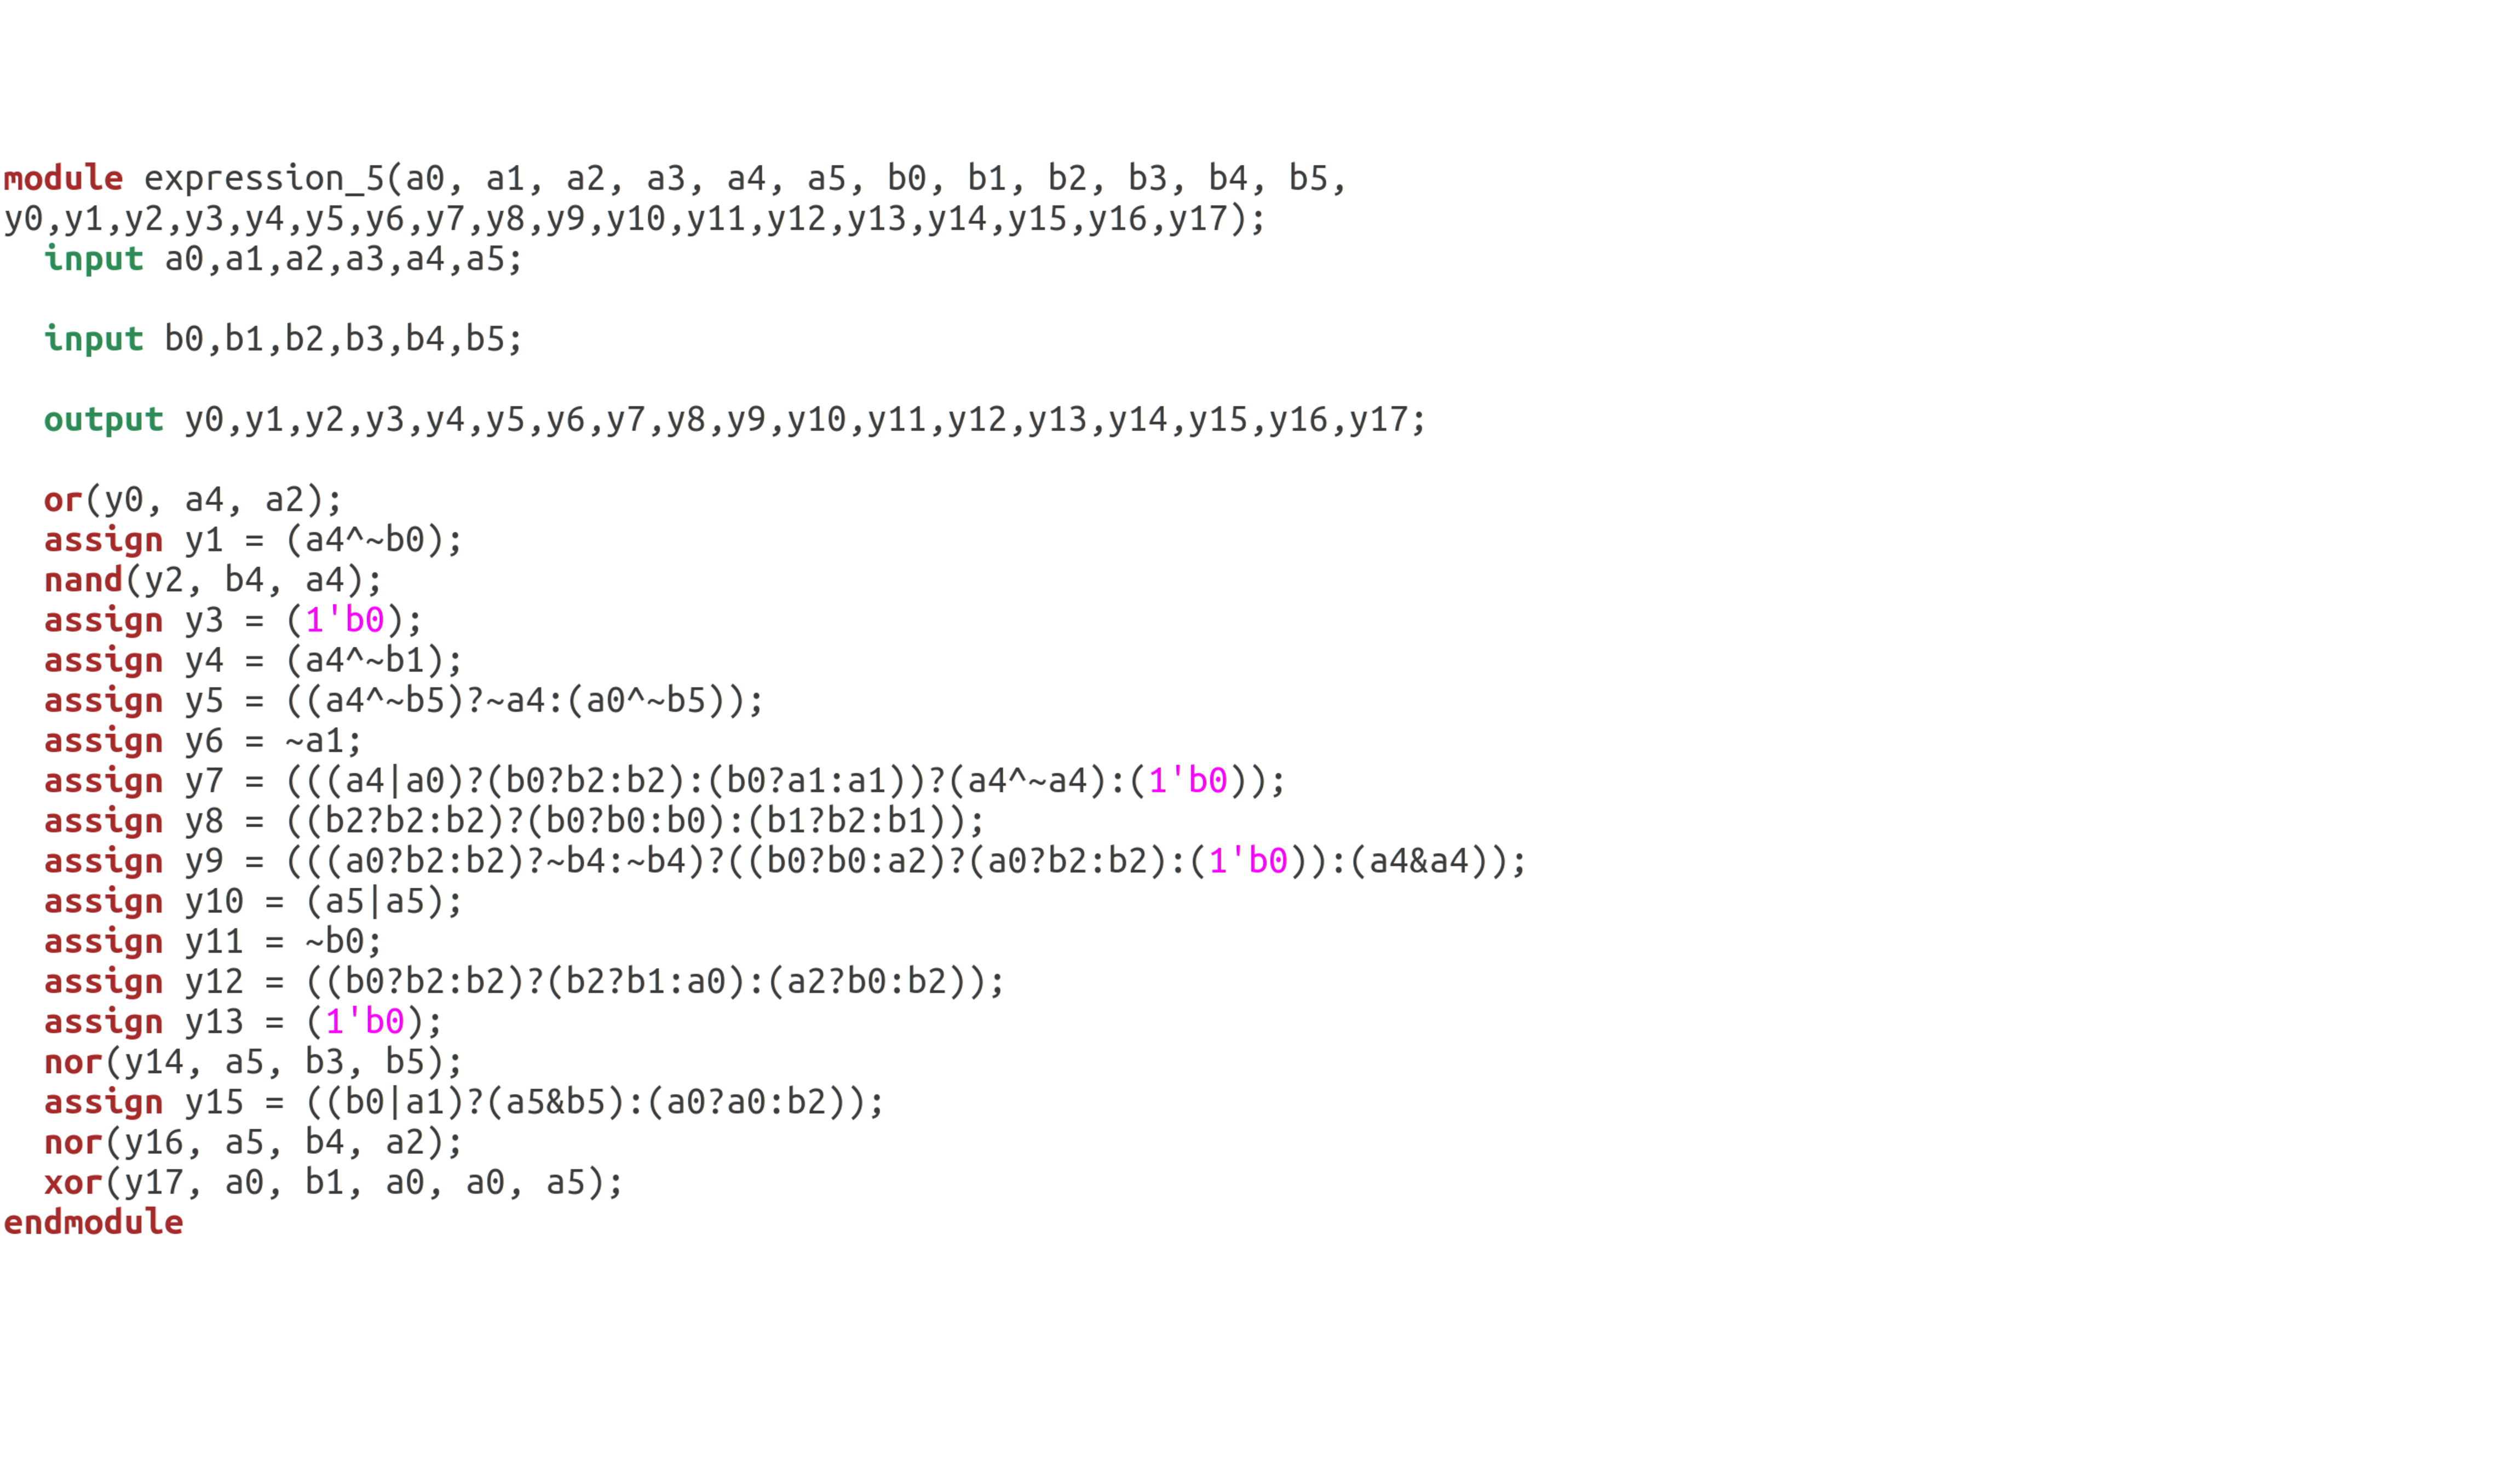
\includegraphics[width=15cm]{MScThesisTemplate/Figs/ex5.pdf}
    \caption{\footnotesize Verilog code of \texttt{general.v}}
\end{figure}
\subsubsection{\texttt{embedded.v}}
Implementation of \texttt{embedded.v} is innovative. It not only contains a main module but also contains a random number of sub-modules. As discussed in design \ref{two degree}, the generation of this kind of file has two degrees of freedom. The number of sub-modules and the number of input port are both bounded at 10. Fig.\ref{fig:hierarchy} shows the hierarchy of this Verilog file. Main-module is the top-level module, and sub-modules are on the same level. The file iteration and statement print approach are almost the same as previous. However, there is a slightly different, printing function of declaring sub-module in main-module needs an addition variable (value of iterator).

\begin{figure}[htbp]
    \centering
    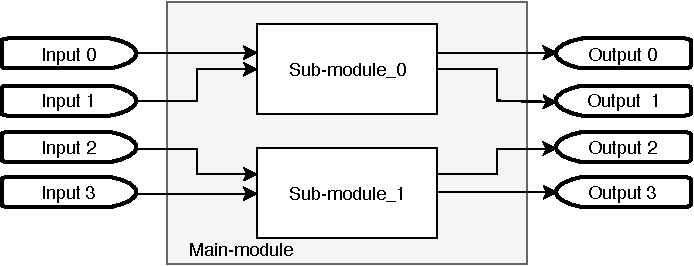
\includegraphics[scale=0.8]{MScThesisTemplate/Figs/embedded_hich.pdf}
    \caption{\footnotesize Hierarchy of \texttt{embedded.v}}
    \label{fig:hierarchy}
\end{figure}
\begin{figure}[htbp]
    \centering
    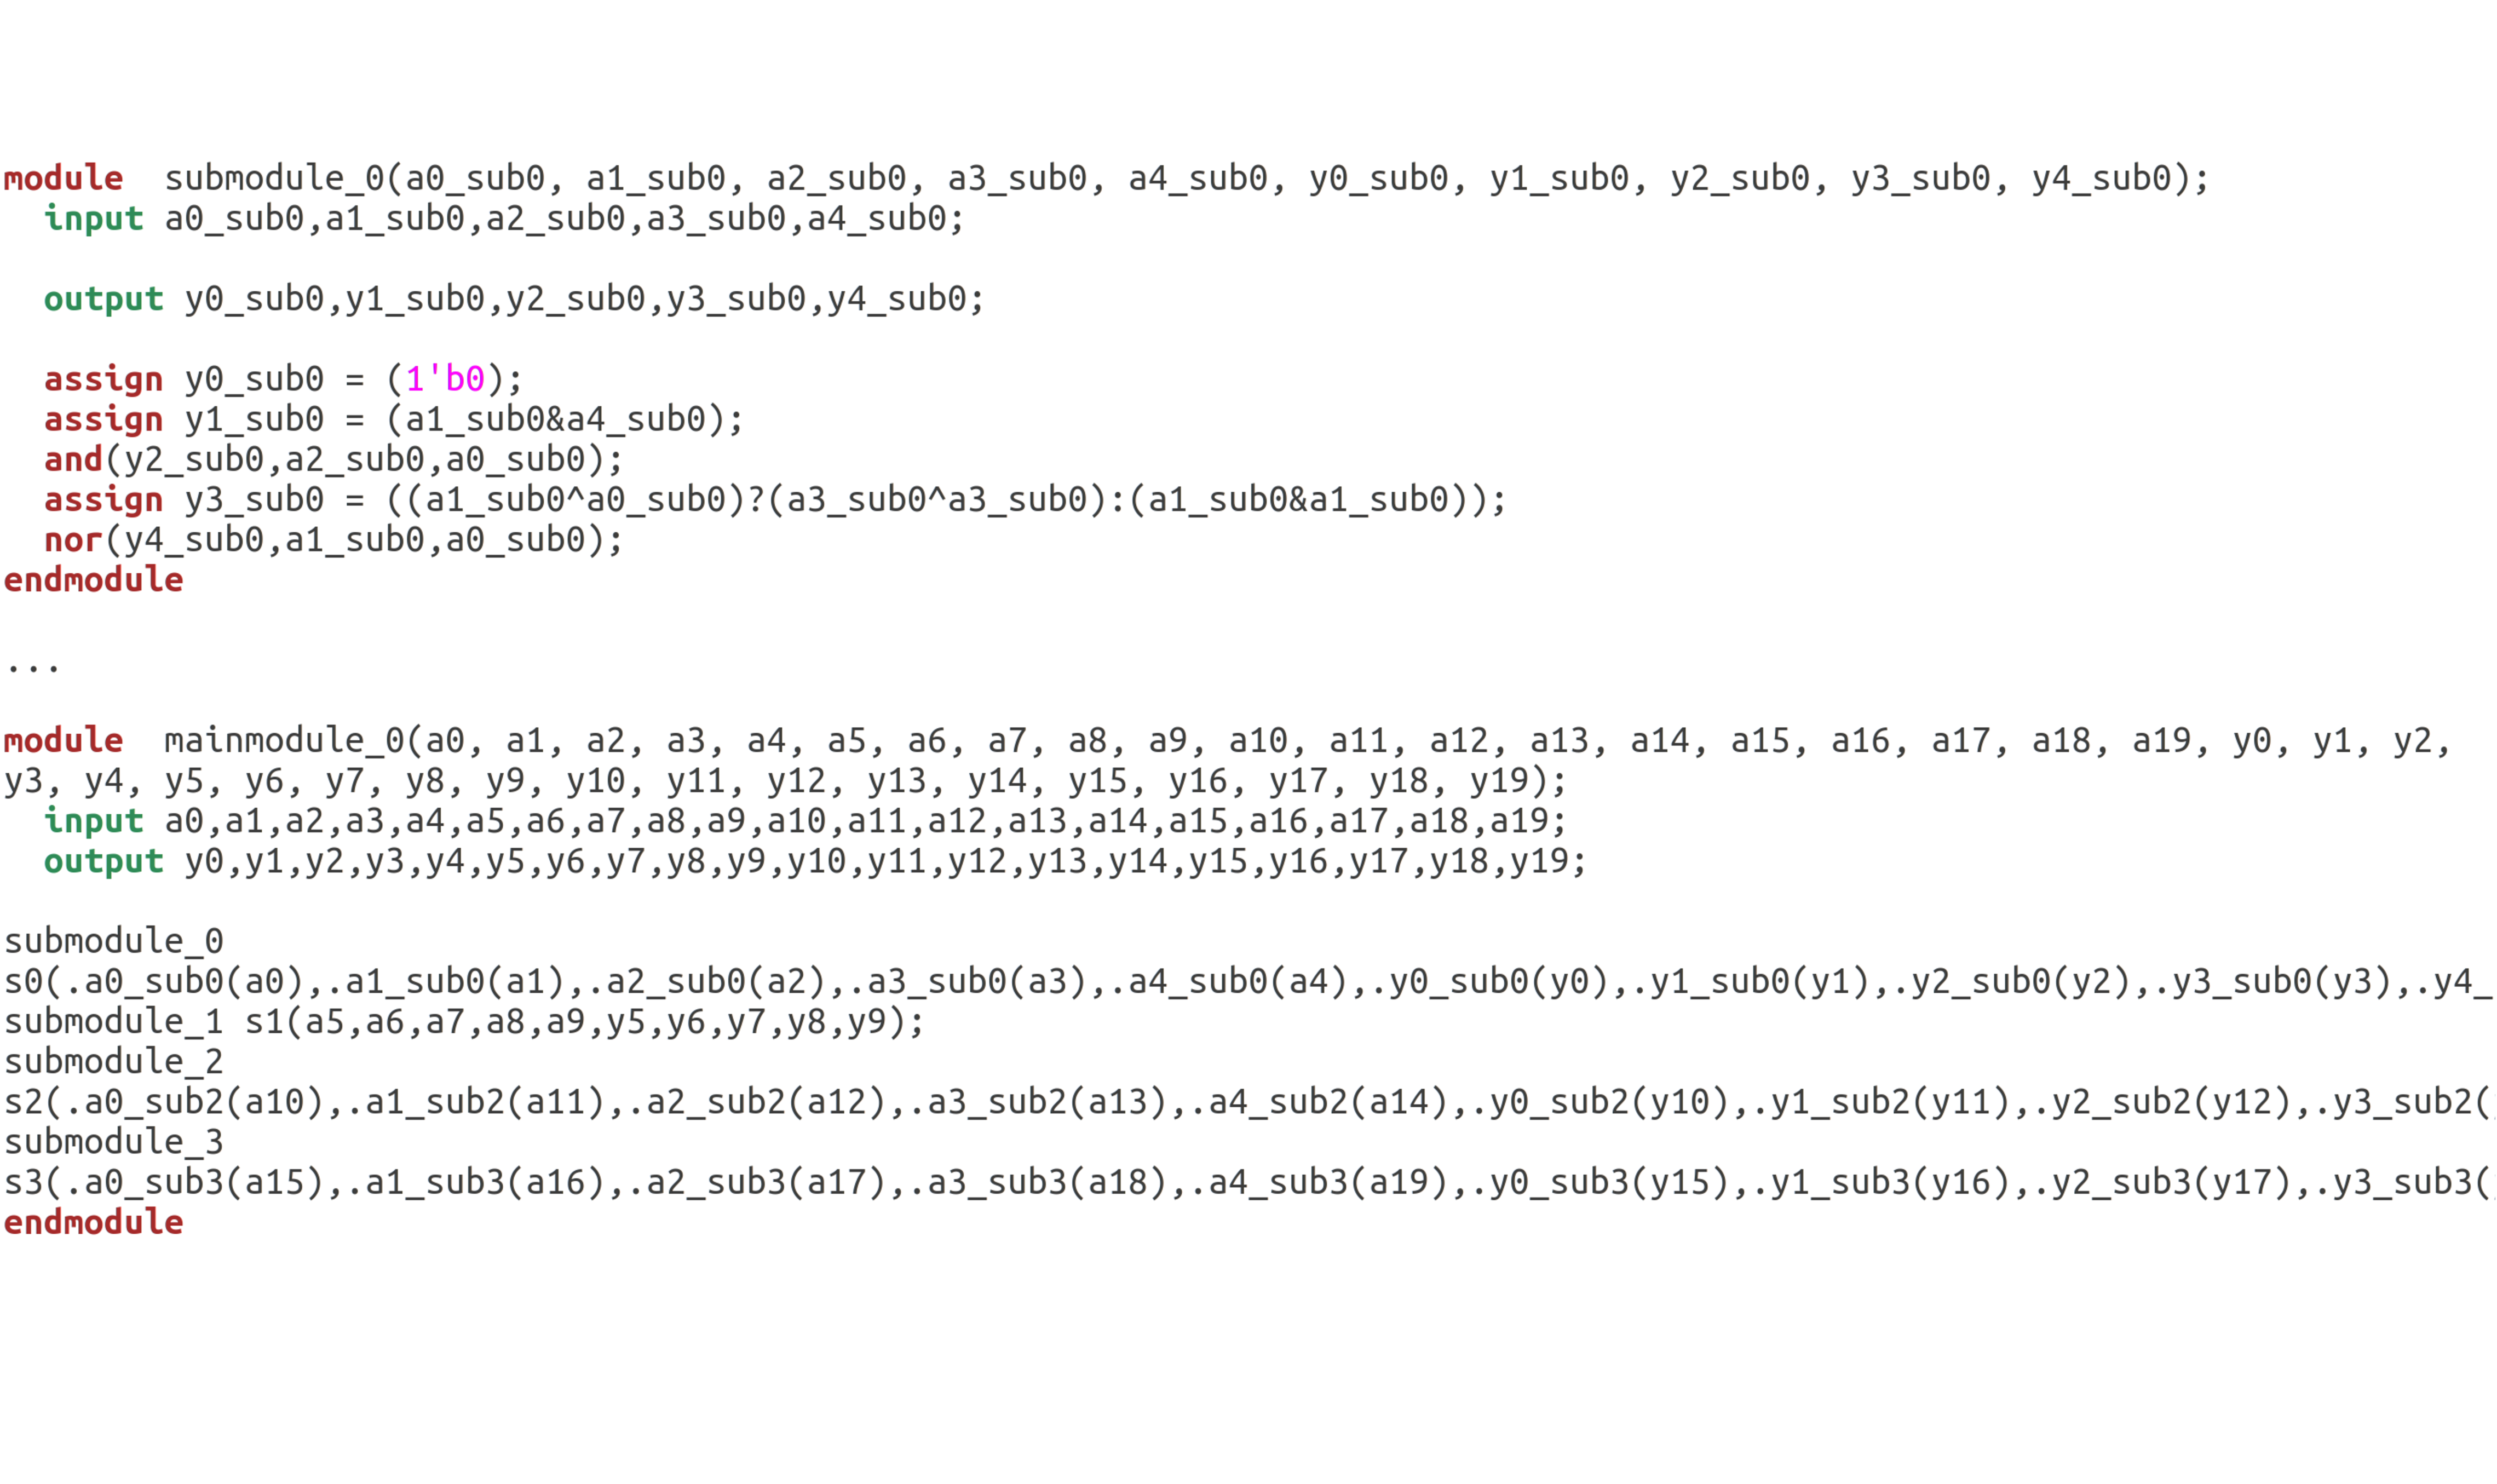
\includegraphics[width=15cm]{MScThesisTemplate/Figs/em0.pdf}
    \caption{\footnotesize Verilog code of \texttt{embedded.v}}
\end{figure}
\subsubsection{\texttt{longer.v}}
The last kind of circuit is a special case of general combinational circuit. It used to stress test HST's capability of large scale input. Hundreds of port is contained in the generated file. It either prints a single enormous module with a large number of port or prints thousands of normal-size modules.

\subsection{Sequential}
Two types of sequential circuit were implemented in this project, \texttt{flipflop.v} and \texttt{FSM.v}. Verilog ''\texttt{alwlays @()}'' statement is widely used in sequential circuit implementation. Contrary to above combination circuit statement printing, sequential circuit print is relatively unique and can not perform recursion. As a result, there is no sequential printing function defined in global environment.

\subsubsection{\texttt{flipflop.v}}
\texttt{flipflop.v} implement an cascade connection of random flip-flops. The number of flip-flops is limited to 10. Memory allocation and iteration uses same method as above combinational circuit generating. According to Verilog syntax, edge trigger signal has two types ''\texttt{posedge}'' and ''\texttt{negedge}''. As a result, there are four different combination of them. The implemented flip-flop will randomly select one triggering combination. Declaration of ''\texttt{alwlays @()}'' block has to be consistent with input edge trigger signals \texttt{CLK} and \texttt{RST} signal. They use same C++ ''\texttt{case}'' judgement variable.  Following step is to print statements in ''\texttt{alwlays @()}'' block. 
\begin{figure}[htb]
    \centering
    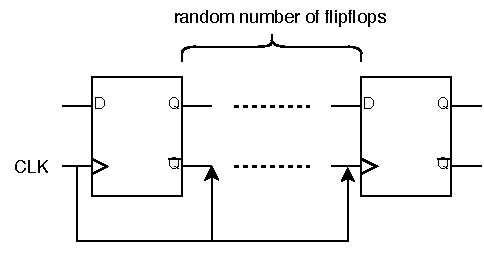
\includegraphics[scale=0.8]{MScThesisTemplate/Figs/ff.pdf}
    \caption{\footnotesize Block diagram of \texttt{flipflop.v}}
    \label{fig:ff}
\end{figure}
\begin{figure}[htb]
    \centering
    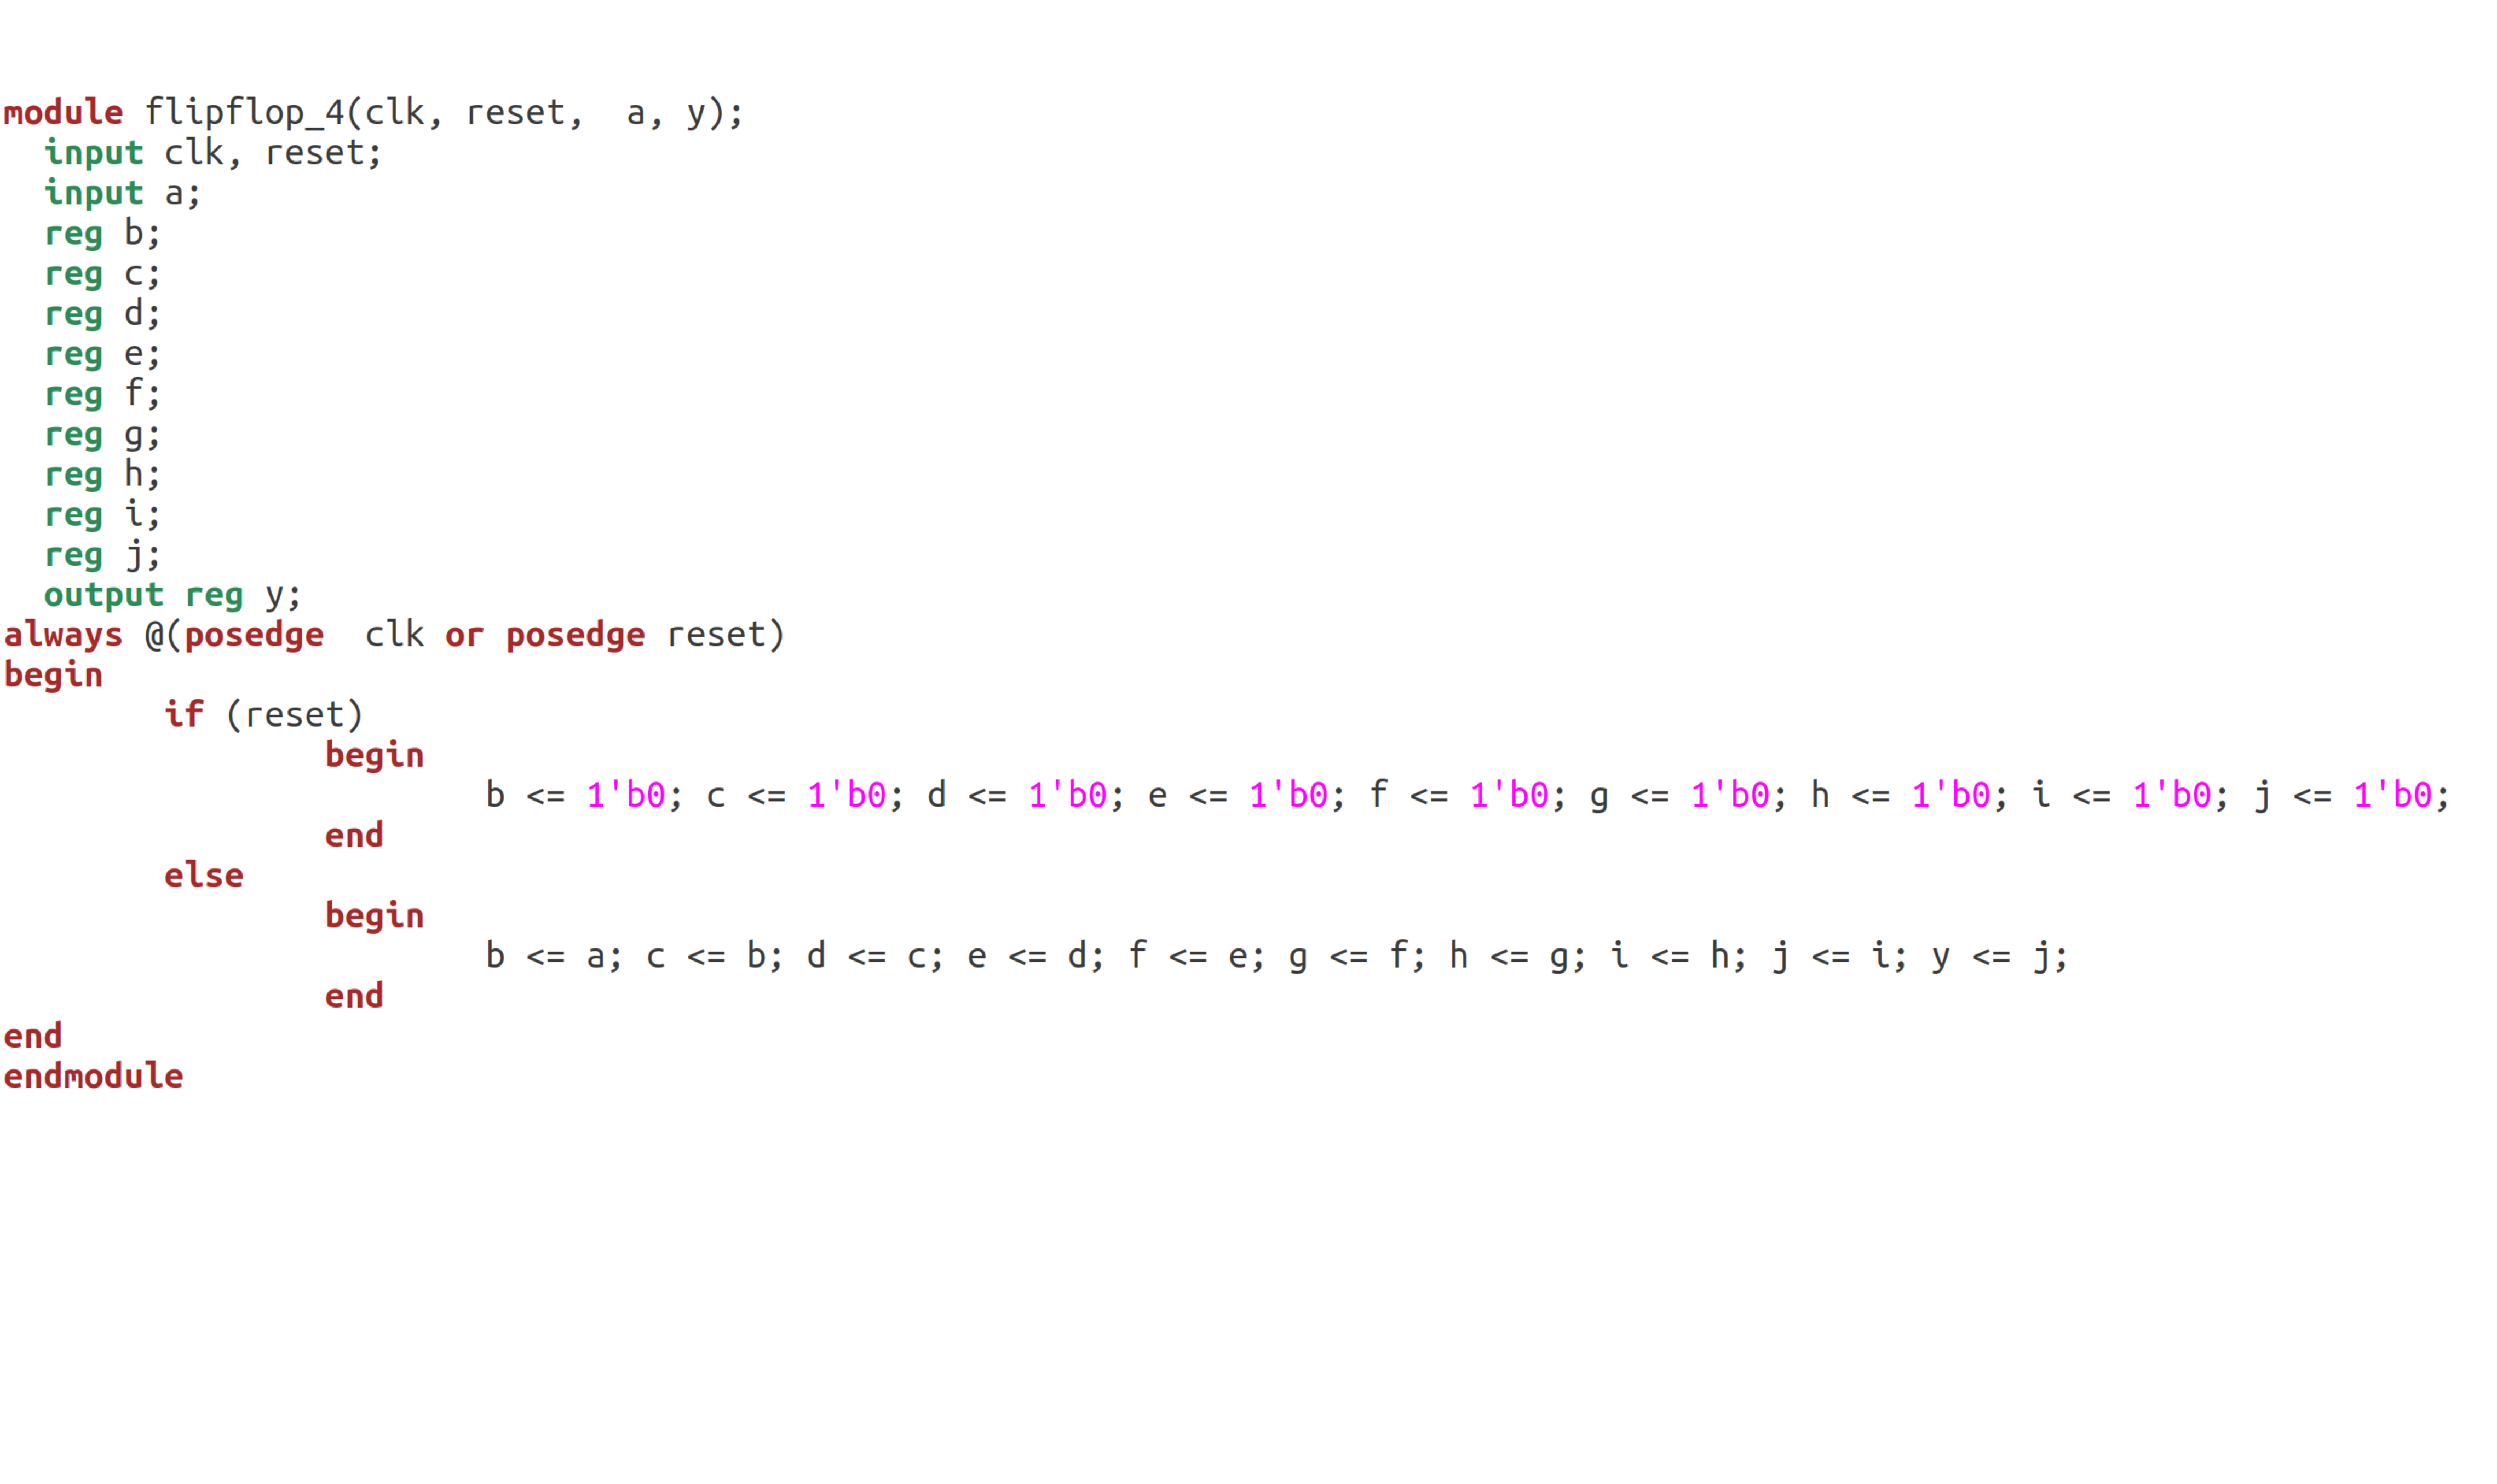
\includegraphics[width=15cm]{MScThesisTemplate/Figs/ff4.pdf}
    \caption{\footnotesize Verilog code of \texttt{flipflop.v}}
\end{figure}

\subsubsection{\texttt{FSM.v}}
The first implementation step of \texttt{FSM.v} is to randomly select the number of state and number of judgements input in a sensitive list. The upper bound of state number is 10. The judgements need to be assigned in the states.  After the specification printing (module name, port declaration and etc), the following step is calling C++ ''\texttt{log2()}'' arithmetic function to calculate bit of ''\texttt{reg}'' variable. For example, four states need a 2-bit ''\texttt{reg}'' variable.

The state transition diagram is shown in the following Fig \ref{fig:fsm}. This implementation of FSM uses two always blocks. The first block is to define the default reset state $S_{0}$. The other block is to perform state transition. If the transition condition is satisfied, it will move to the next state. Otherwise, it will remain in the present state. For last state $S_{n}$, it will randomly move to one of the previous states.

For the final output port printing, it is randomly selected as state-decided or state/input-decided. This produces a random selection between Moore state machine or Mealy state machine. Same as above procedure, ''endmodule'' will be printed at the end of the file.

\begin{figure}[htb]
    \centering
    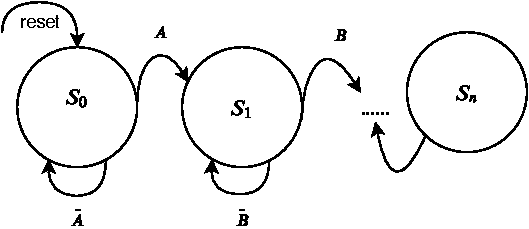
\includegraphics[scale=0.8]{MScThesisTemplate/Figs/FSM.pdf}
    \caption{\footnotesize State transition diagram of \texttt{FSM.v} }
    \label{fig:fsm}
\end{figure}
\begin{figure}[htbp]
    \centering
    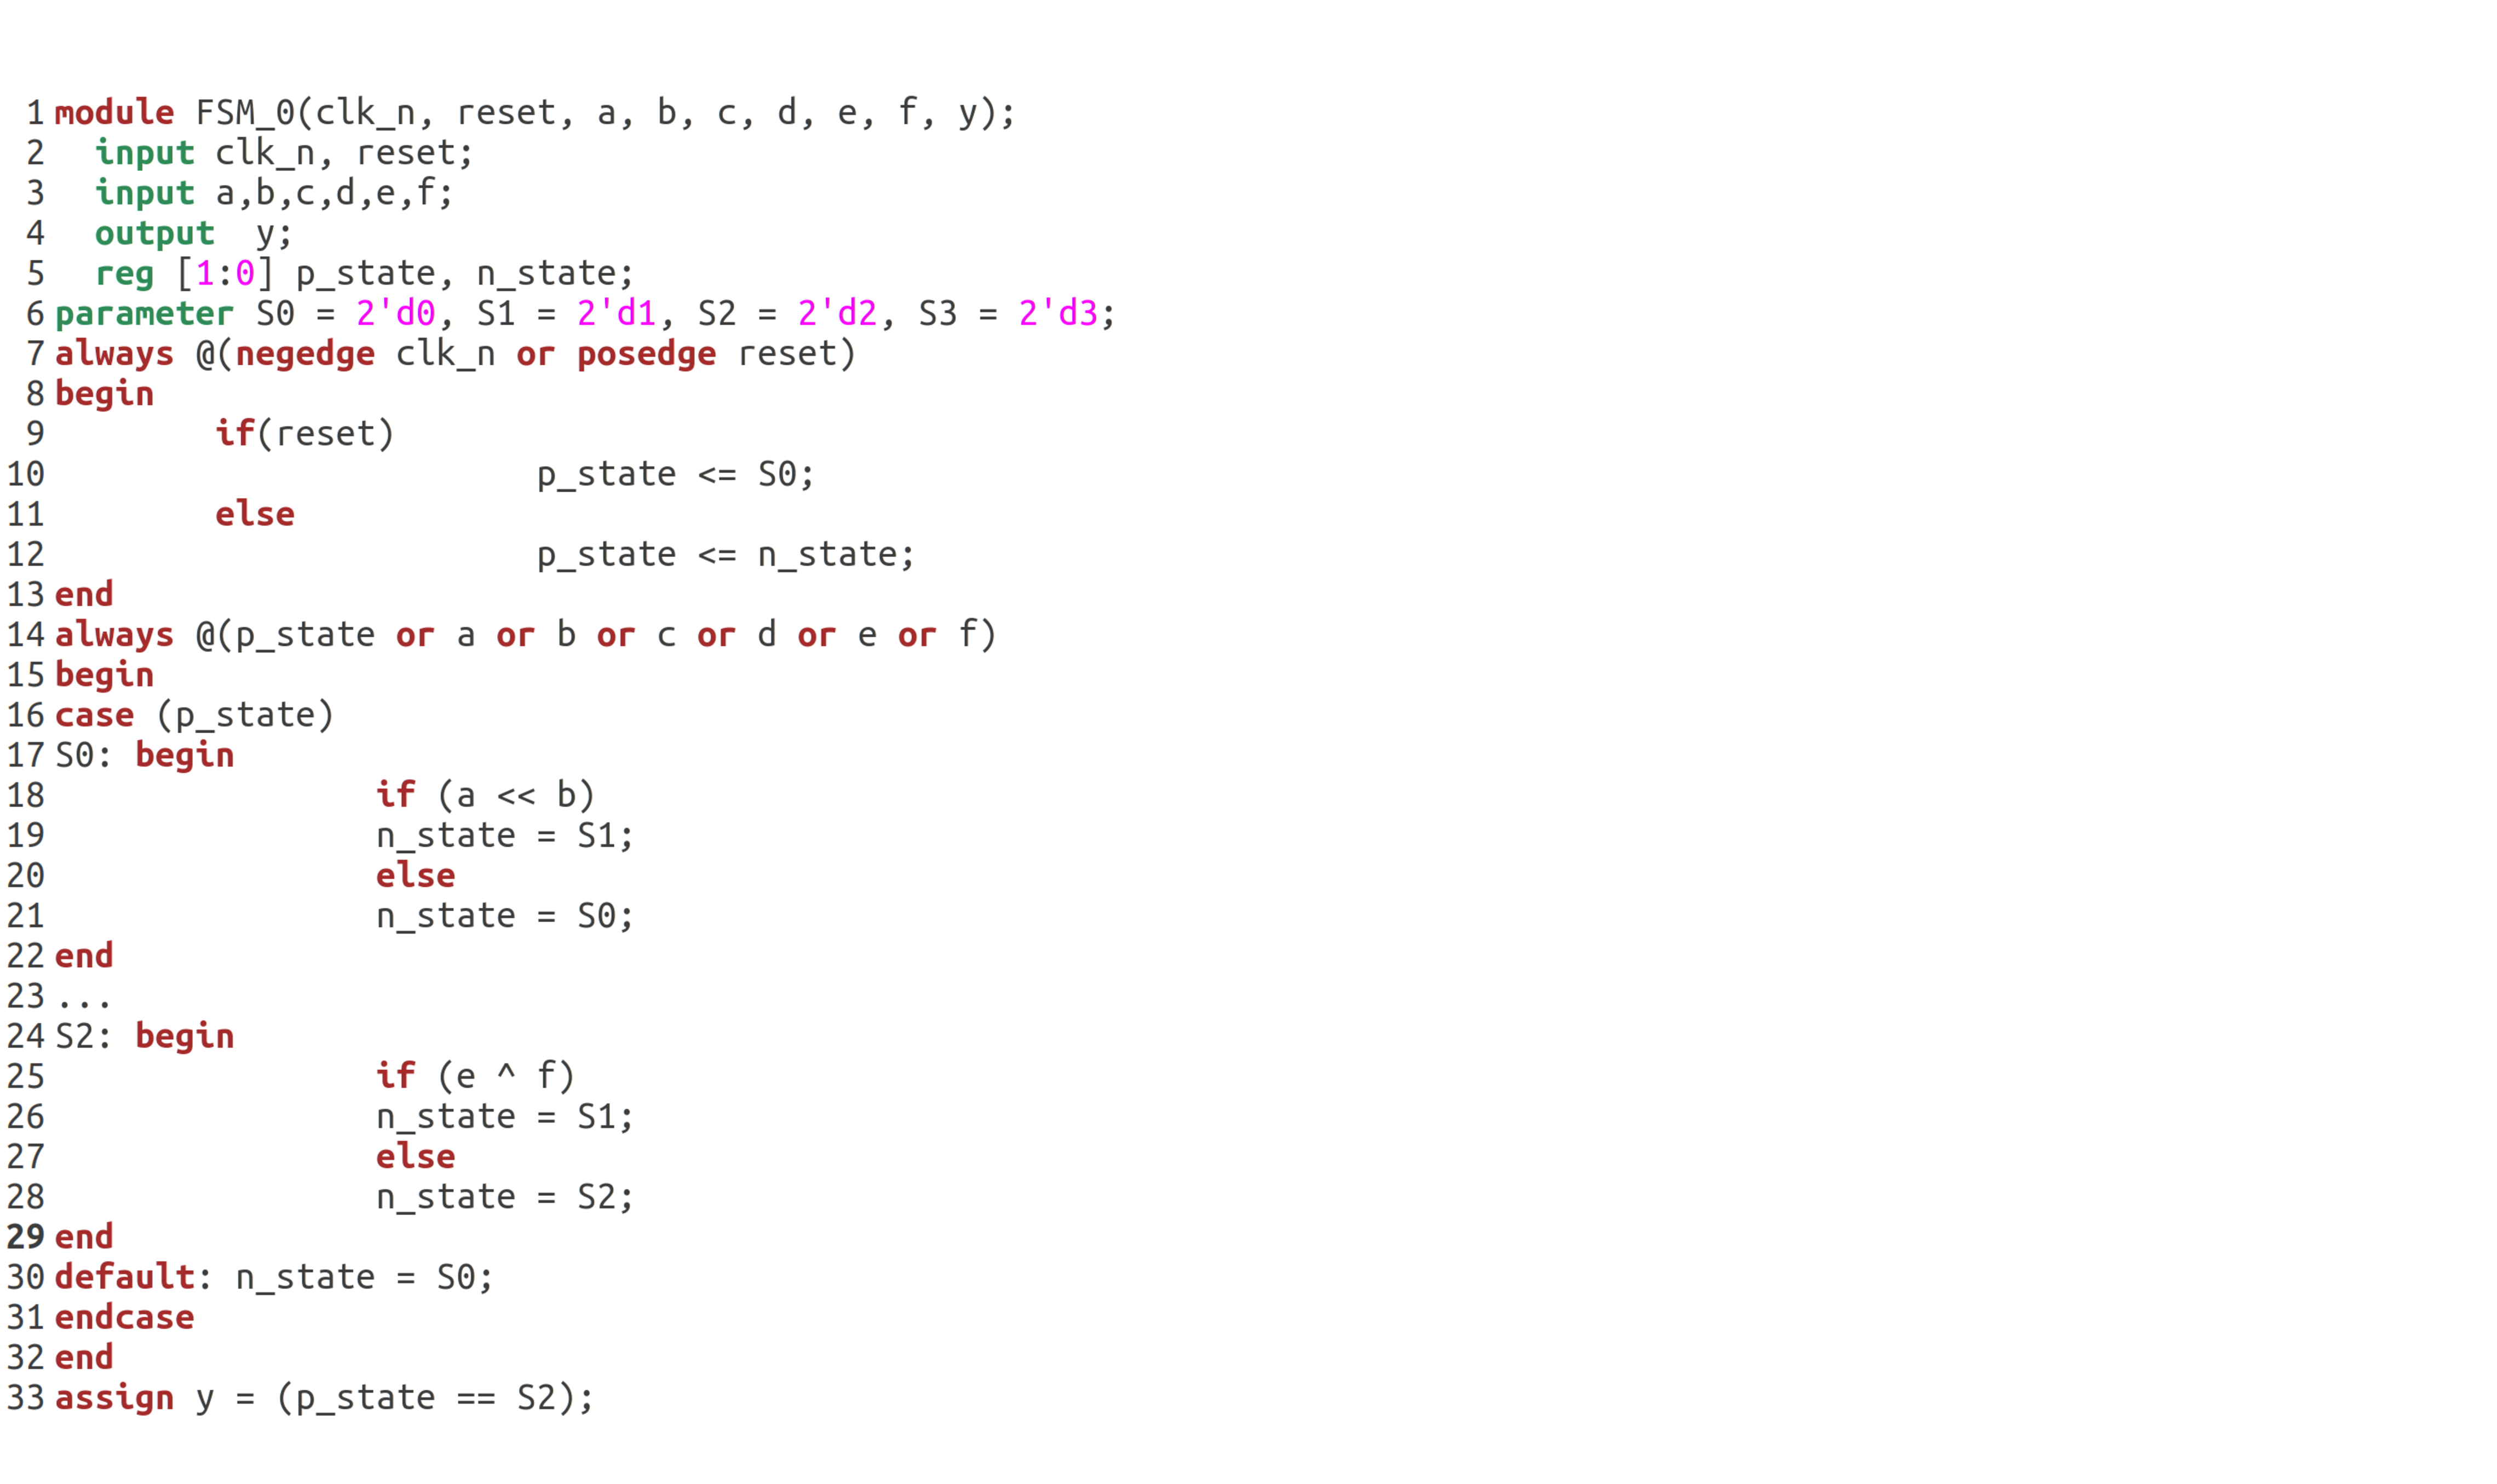
\includegraphics[width=15cm]{MScThesisTemplate/Figs/fsm0.pdf}
    \caption{\footnotesize Verilog code of \texttt{FSM.v}}
\end{figure}